\documentclass[newPxFont,numfooter,sectionpages]{beamer}
\usepackage[utf8]{inputenc}
\usepackage[T2A]{fontenc}
\usepackage[russian]{babel}
\usepackage{eufrak}
\usetheme{sthlm}
\usepackage{pgfplots}
\usepackage{cancel}

\usepackage{multirow}
\usepackage[normalem]{ulem}
\useunder{\uline}{\ul}{}

%\usepackage{wrapfig}
\usepackage{graphicx}
\usepackage{subcaption}
%\graphicspath{{pictures/}}
\DeclareGraphicsExtensions{.pdf, .jpg, .png}

\usepackage{geometry} %способ ручной установки полей
%\geometry{top=4mm} %поле сверху
\geometry{bottom=4mm} %поле снизу
\geometry{left=4mm} %поле справа
\geometry{right=4mm} %поле слева

\title{Вывод уравнений движения мобильного манипулятора}
\subtitle{}
%\date{\today}
\author{Автор: Дема Николай\\Преподаватель: Колюбин Сергей Алексеевич}
\institute{\small{Курс: Динамика Робототехнических систем\\ \ Университет ИТМО}}

\begin{document}

\maketitle

% 1
\begin{frame}{Содержание}
	% For longer presentations use hideallsubsections option
	\tableofcontents[hideallsubsections]
	\begin{itemize}
		\item[-] Что такое мобильный манипулятор 
        \item[-] Описание кинематики мобильных платформ
        \item[-] Описание кинематики манипулятора
        \item[-] Обзор методов описания динамики
        \item[-] Вывод уравнения динамики мобильного манипулятора	
	\end{itemize}	
\end{frame}

% 2
\begin{frame}{Что такое мобильный манипулятор}
	\begin{figure}[H]
		\center
		\renewcommand{\figurename}{}
		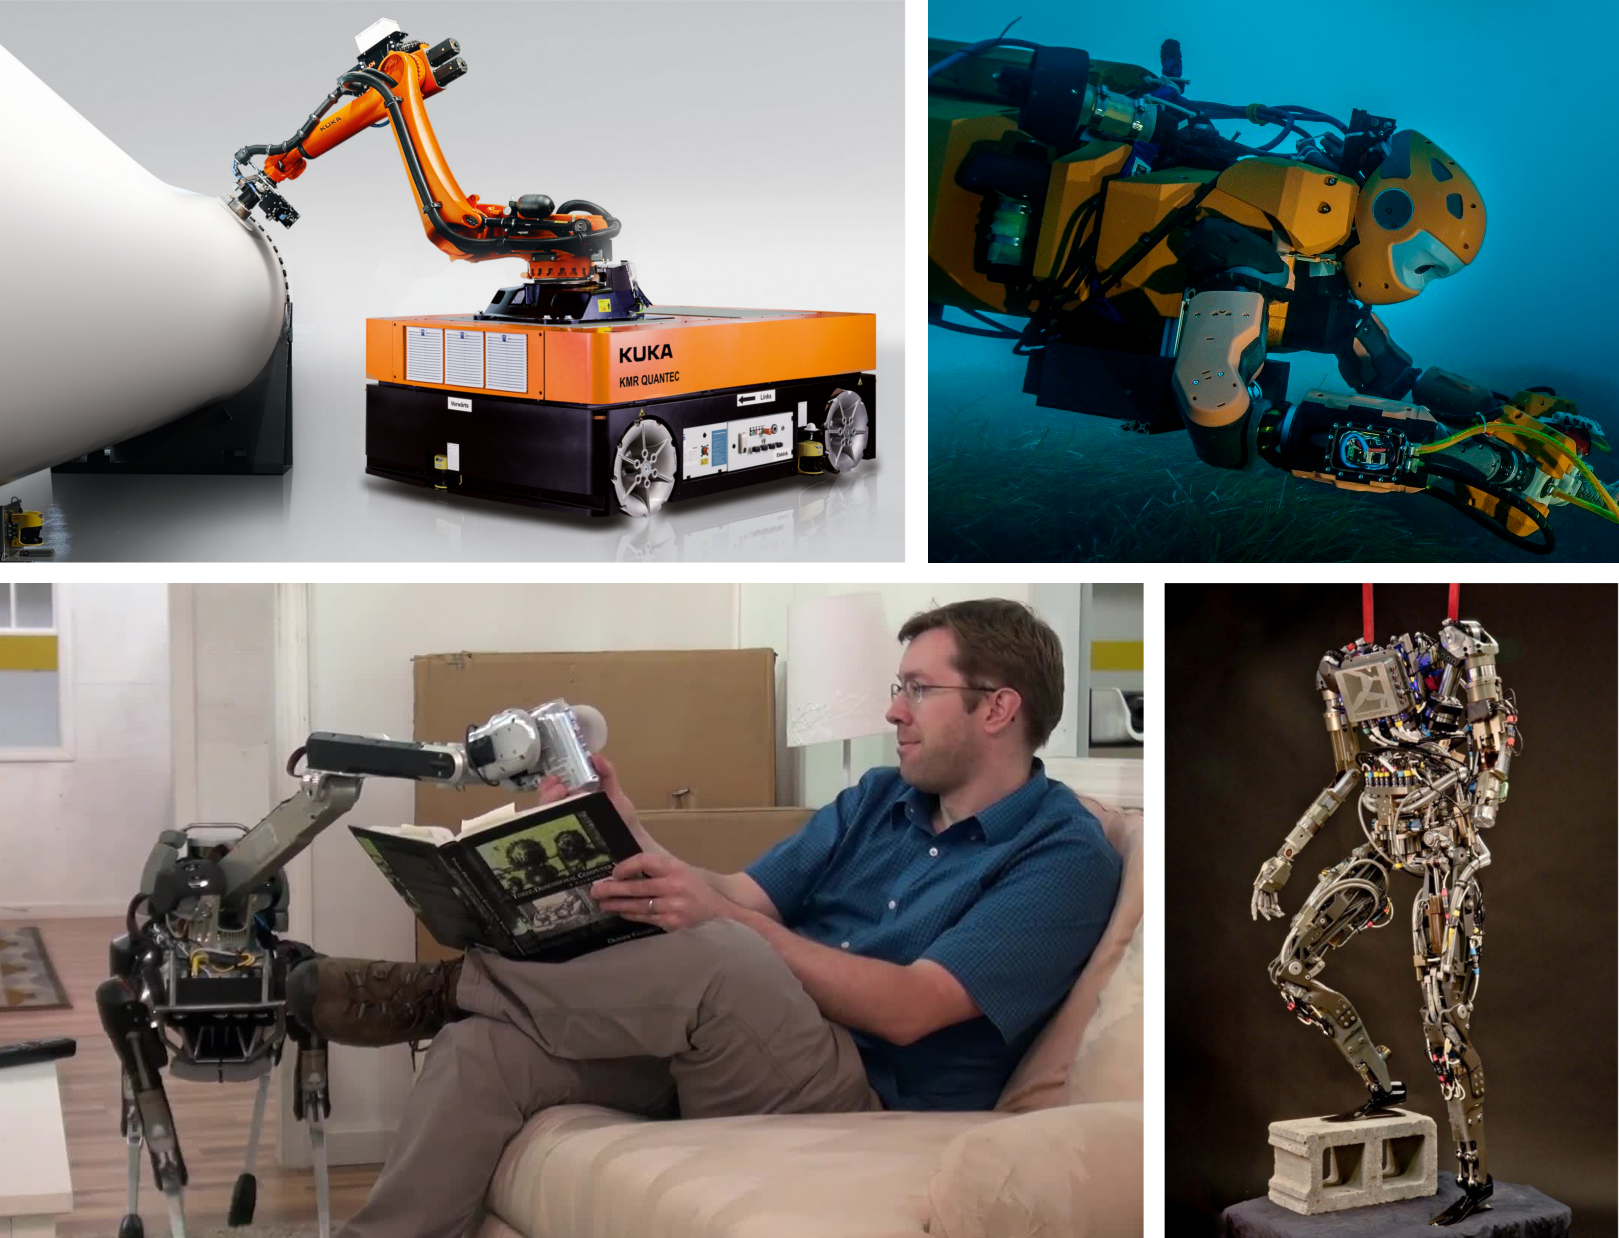
\includegraphics[width=0.9\linewidth]{pic/mm_all.png}
		%\caption{Оси координат двух соседних звеньев}
		\label{fig:scr1}
	\end{figure}
\end{frame}
%\cOrange{Заданы:}

% 3
\begin{frame}{Описание кинематики мобильных платформ}
\ \\

	\begin{minipage}{0.42\textwidth}
	\begin{flushleft} 
	\begin{figure}[H]
		\center
		\renewcommand{\figurename}{}
		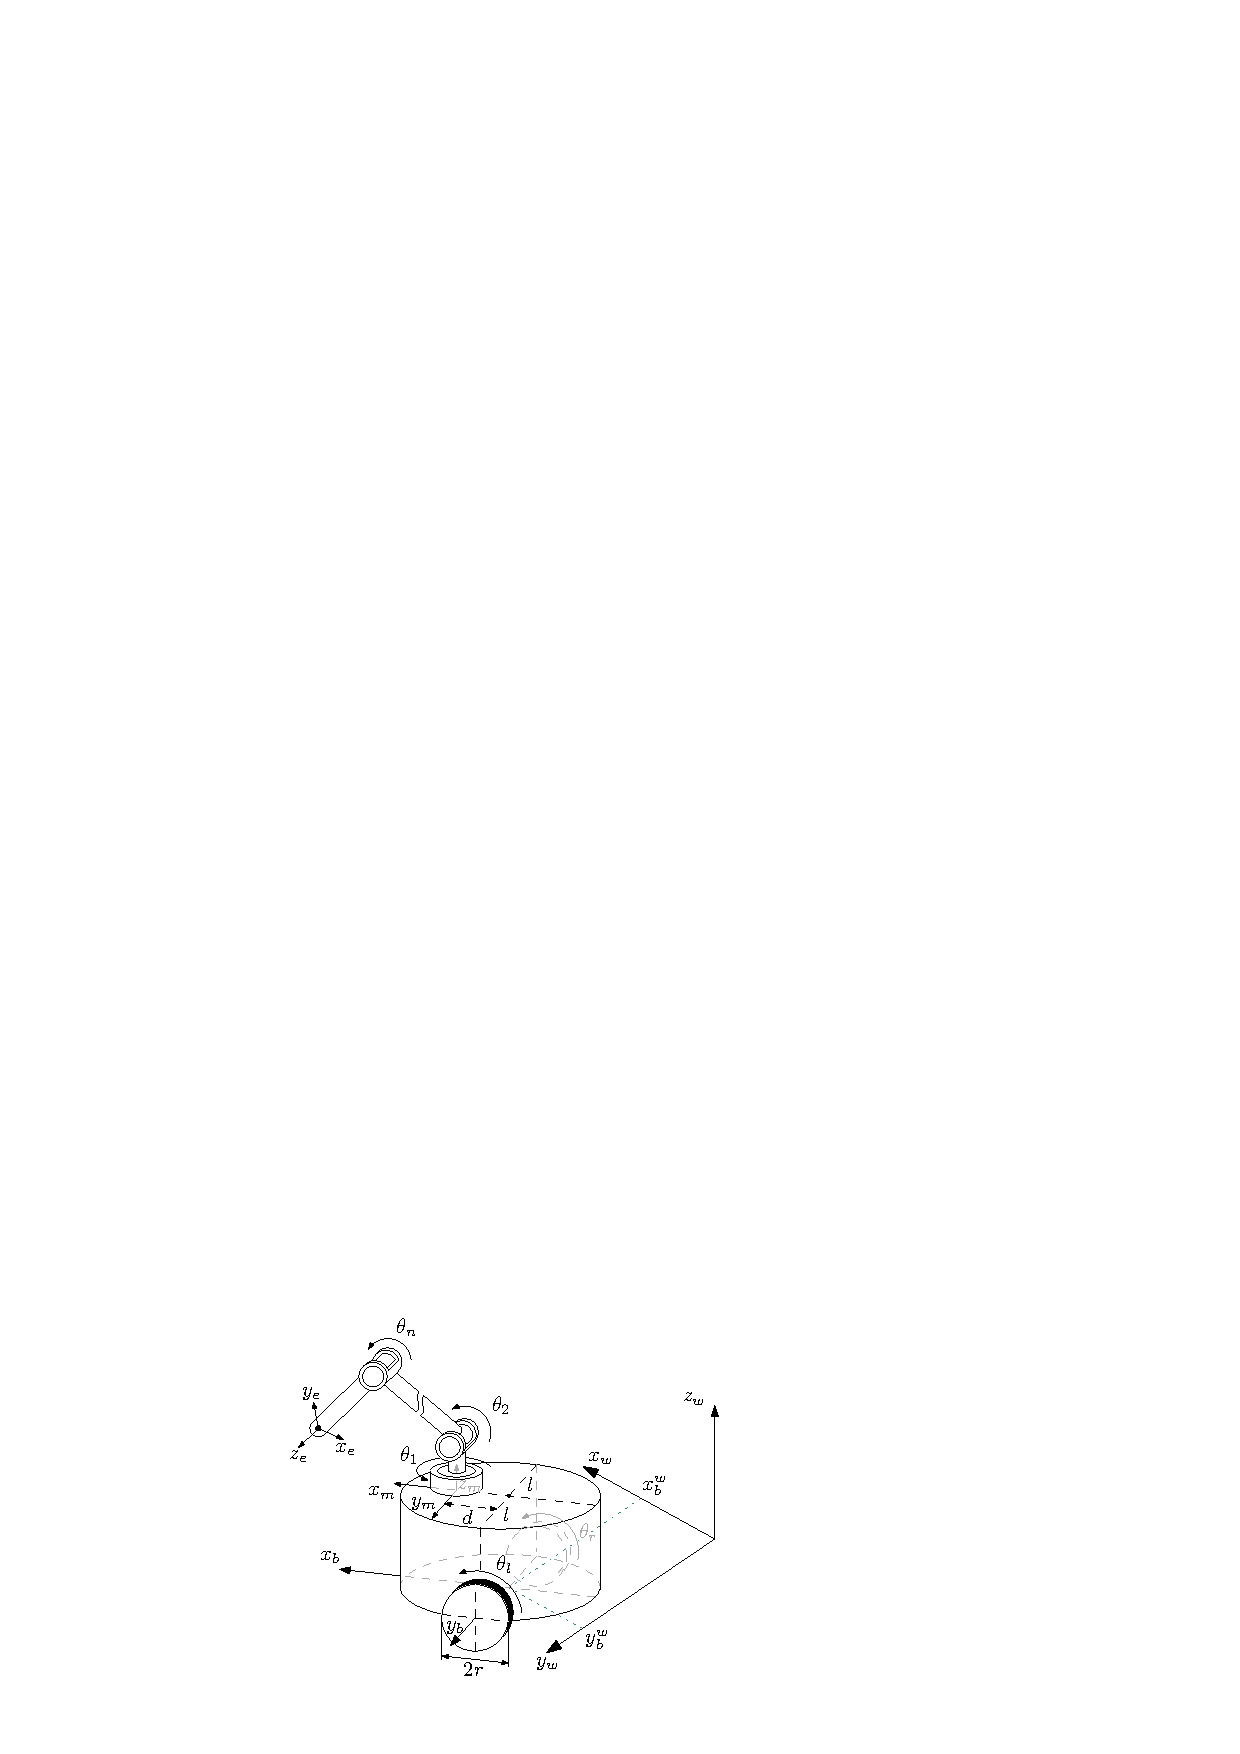
\includegraphics[width=1.3\linewidth]{pic/MM3.pdf}
		%\caption{Оси координат двух соседних звеньев}
		\label{fig:scr1}
	\end{figure}		
	\end{flushleft} 
	\end{minipage}
	%\hfill	
		\begin{minipage}{0.56\textwidth}
		%\begin{center}
			\begin{equation}
				{^wr_e} = F(q),\ q = [q_b^T,q_m^T]^T
				\tag{1} \label{eq:1}
			\end{equation}
			\begin{equation}
			q_b = [x^w_b, y^w_b, \psi]^T
			\tag{2} \label{eq:2}
			\end{equation}
			\begin{equation}
			q_m = [q_{m1}, q_{m2}, ..., q_{mn_m}]^T
			\tag{3} \label{eq:3}
			\end{equation}
			\begin{equation}
			{^w\dot{r}_e} = \left(\frac{\partial F}{\partial q_b}\right)\dot{q}_b + \left(\frac{\partial F}{\partial q_m}\right)\dot{q}_m
			\tag{4} \label{eq:4}
			\end{equation}
			\begin{equation}
			\dot{q}_b = G(q_b)u_{q_b}, \ \ |u_{q_b}| \leqslant |\dot{q}_b|
			\tag{5} \label{eq:5}
			\end{equation}
		%\end{center}
	\end{minipage}
	\begin{center}
	\begin{minipage}{0.8\textwidth}
	\begin{center}
	
	$G(q_b)$ --- определяется типом используемой базы
	\end{center}
	\end{minipage}
	\end{center}
	
\end{frame}

% 4
\begin{frame}{Описание кинематики мобильных платформ}

	\begin{center}
		\begin{minipage}[b]{0.9\textwidth}
			Движение базы такого типа ограничивается стационарными неголономными связями, которые в общем виде могут быть представлены как:
	
			\begin{equation}
				A(q_b)\dot{q}_b = 0, A \in R^{s\times|q_b|}
				\tag{6} \label{eq:6}
			\end{equation}

			\noindent
			где $A(q_b)$ --- прямоугольная матрица, элементы которой являются функциями обобщённых координат, $s$ --- определяется количеством накладываемых на систему неголономных связей. Для рассматриваемой платформы:
			
			\begin{equation}
				\dot{x}^w_b\sin(\psi) - \dot{y}^w_b\cos(\psi) = 0
				\tag{7} \label{eq:7}
			\end{equation}
			
			\begin{equation}
				\dot{x}^w_b\cos(\psi) + \dot{y}^w_b\sin(\psi) = \frac{r}{2}(\dot{\theta}_r + \dot{\theta}_l)
				\tag{8} \label{eq:8}
			\end{equation}	
		\end{minipage}
	\end{center}
\end{frame}

% 5
\begin{frame}{Описание кинематики мобильных платформ}

	\begin{center}
		\begin{minipage}[b]{0.9\textwidth}
			Тогда для:
	
			\begin{equation}
				q_b = 
				\begin{bmatrix}
				x^w_b & y^w_b & \theta_r & \theta_l
				\end{bmatrix}^T
				\tag{9} \label{eq:9}
			\end{equation}

			\noindent
			с учетом (7) и (8):
			\begin{equation}
			A(q_b) = 
			\begin{bmatrix}
			-\sin(\psi) & \cos(\psi) & 0 & 0\\[1mm]
			\cos(\psi) & \sin(\psi) & -\frac{r}{2} & -\frac{r}{2}\\[1mm]
			\end{bmatrix}
			\tag{10} \label{eq:10}
			\end{equation}
			Матрица $G(q_b)$ из (\ref{eq:5}) может быть сформирована из множества линейно независимых векторов входящих в нуль-пространство матрицы $A(q)^*$, т.е.:
			
			\begin{equation}
				G(q_b)^T A(q_b)^T = 0
				\tag{11} \label{eq:11}
			\end{equation}
			
		\end{minipage}
	\end{center}
	
	\tiny{$^*$Li Z., Ge S. S. Fundamentals in Modeling and Control of Mobile Manipulators.\\ \ Vol. 49. —
CRC Press, 2013.\\ \ }
\end{frame}

% 6
\begin{frame}{Описание кинематики мобильных платформ}

	\begin{center}
		\begin{minipage}[b]{0.9\textwidth}
			Полная кинематическая модель мобильной платформы с учетом смещения точки крепления манипулятора относительно начала системы координат:
			
		\end{minipage}
		\begin{equation}
			\begin{bmatrix}
			\dot{x}^w_b\\[1mm] \dot{y}^w_b\\[1mm] \dot{\psi}\\[1mm] \dot{\theta}_r\\[1mm] \dot{\theta}_l
			\end{bmatrix} = 
			\begin{bmatrix}
			\frac{r}{2}(\cos(\psi) - dl\sin(\psi)) & \frac{r}{2}(\cos(\psi) + dl\sin(\psi))\\[1mm]
			\frac{r}{2}(\sin(\psi) + dl\cos(\psi)) & \frac{r}{2}(\sin(\psi) - dl\cos(\psi))\\[1mm]
			\frac{r}{2l} & -\frac{r}{2l}\\[1mm]
			1 & 0\\[1mm]
			0 & 1\\[1mm]
			\end{bmatrix}
			\begin{bmatrix}
			\dot{\theta}_r\\[1mm] \dot{\theta}_l
			\end{bmatrix}
			\tag{12} \label{eq:12}
		\end{equation}
	\end{center}
\end{frame}

% 7
\begin{frame}{Описание кинематики манипулятора}

	\begin{center}
		\begin{minipage}[b]{0.9\textwidth}
			Для описания преобразований систем координат последовательного манипулятора можно воспользоваться соглашением Денавита-Хартенберга:
		\begin{figure}[H]
		\center
		\renewcommand{\figurename}{}
		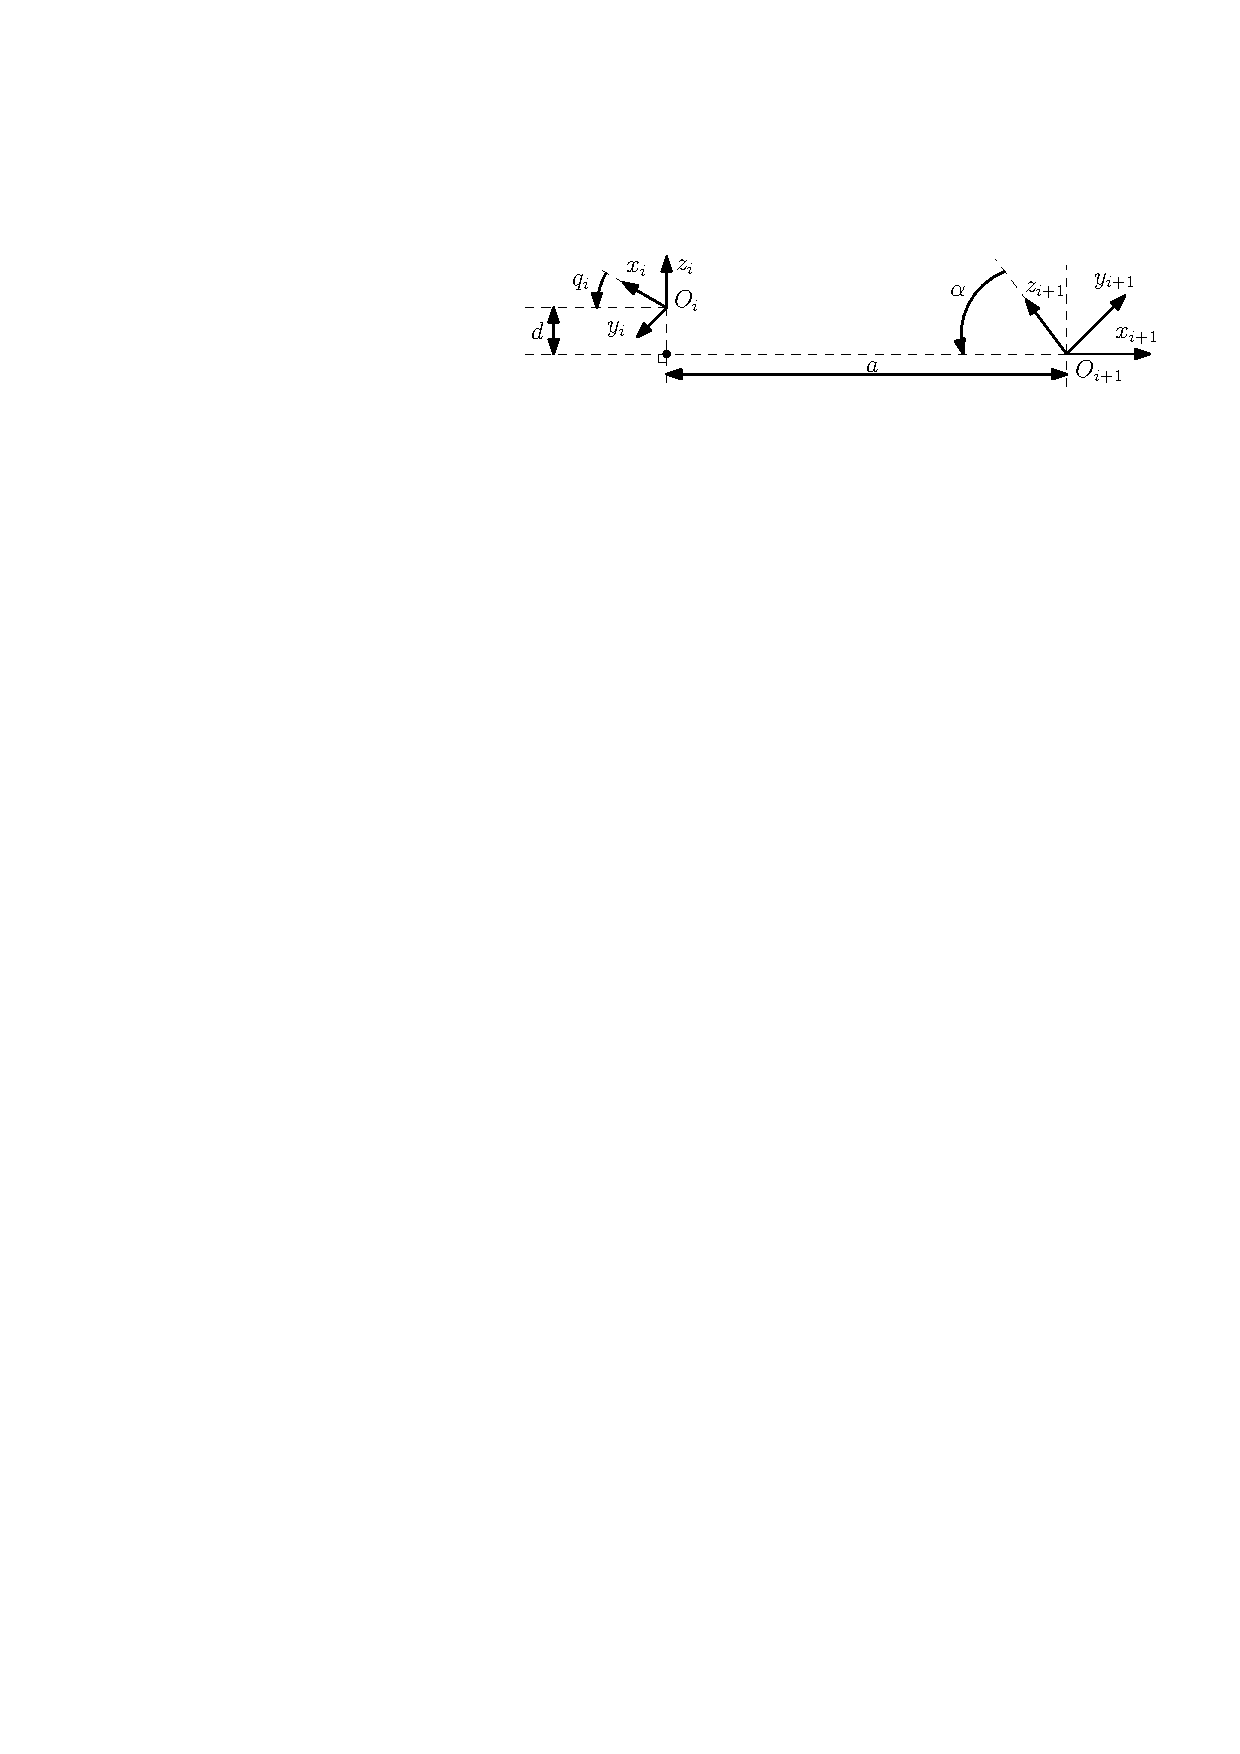
\includegraphics[width=0.8\linewidth]{pic/DH.pdf}
		%\caption{Оси координат двух соседних звеньев}
		\label{fig:scr1}
	\end{figure}
	
	\[
^{i-1}H_i =
	\begin{bmatrix}
		c_{q_{mi}} & 	-s_{q_{mi}}c_{\alpha_i} & 	s_{q_{mi}}s_{\alpha_i}	&	a_ic_{q_{mi}}\\
		s_{q_{mi}} & 	c_{q_{mi}}c_{\alpha_i} &	-c_{q_{mi}}s_{\alpha_i} &	a_is_{q_{mi}}\\
		0				&	s_{\alpha_i} 						&	c_{\alpha_i}					& 	d_i\\
		0				&	0									&	0								&	1
	\end{bmatrix} \tag{13} \label{eq:13}
\]

\begin{equation}
^{0}H_n(q_{m}) = \prod_{i=1}^{n} \left(^{i-1}H_i\right).
\tag{14} \label{eq:14}
\end{equation}
			
		\end{minipage}
	\end{center}
\end{frame}

% 8
\begin{frame}{Описание кинематики манипулятора}

	\begin{center}
		\begin{minipage}[b]{0.9\textwidth}
			Прямая задача кинематики для  манипулятора последовательной кинематики может быть решена, как:
\begin{equation}
^mr_e = {^0H}_n(q_{m})\mathbf{O},\,\, \mathbf{O}\ \text{--- нулевой вектор} (n_m\times 1)
\tag{15} \label{eq:15}
\end{equation}
	
Элемент $\left(\frac{\partial F}{\partial q_m}\right)$ из ур. (4) является Якобианом $J$ манипулятора и может определятся как:

\begin{equation}
J(q_m) = 
\begin{bmatrix}
J_1 & J_2 & ... & J_{n_m}
\end{bmatrix}
\tag{16} \label{eq:16}
\end{equation}

\noindent
где $J_i$ --- составляющая якобиана для i-го сочленения манипулятора, для вращательного сочленения определяется как:
\begin{equation}
J_i = 
\begin{bmatrix}
z^0_{i-1} \times (p^0_{n_m} - p^0_{i-1})\\[1mm]
z^0_{i-1}
\end{bmatrix}
\tag{17} \label{eq:17}
\end{equation}
		\end{minipage}
	\end{center}
\end{frame}

% 9
\begin{frame}{Обзор методов описания динамики}

	\begin{center}
		\begin{minipage}[b]{0.9\textwidth}
			Вывод уравнений динамики для мобильных манипуляторов в общем является нетривиальной задачей ввиду огромного разнообразия систем такого типа.
			\ \\
			
			Среди наиболее распространенных методов можно выделить основанные на уравнениях Эйлера---Лагранжа, Ньютона---Эйлера, Гиббса-Аппеля и Кейна.
		\end{minipage}
	\end{center}
\end{frame}


% 10
\begin{frame}{Обзор методов описания динамики (Эйлер-Лагранж)}

	\begin{center}
		\begin{minipage}[b]{0.9\textwidth}
		Получение уравнений динамики методом Эйлера-Лагранжа отличается простотой и единством подхода, обеспечивает строгое описание состояния системы, и может быть использовано для разработки усовершенствованных законов управления и способов описания самих систем.
		\ \\
		
		Для получения уравнений движения методом Эйлера-Лагранжа в контексте мобильных колесных платформ используют его вариант, включающий в уравнения неопределенные множители Лагранжа для учета неголономных связей. 
		\end{minipage}
	\end{center}
\end{frame}

% 11
\begin{frame}{Обзор методов описания динамики (Гиббс-Аппель)}

	\begin{center}
		\begin{minipage}[b]{0.9\textwidth}
		В основе подхода лежит функция "энергии ускорения" Гиббса которая для i-го звена системы может быть выражена как:

\begin{equation}
S_i = \frac{m_i a_i^2}{2}  + \frac{\varepsilon_i^T I_i \varepsilon_i}{2}  + 2 (\omega_i \times I_i \omega_i) \varepsilon_i
\tag{18} \label{eq:18}
\end{equation}

Для получения уравнений движения, выраженных относительно обобщенных координат рассчитывается функция Гиббса-Аппеля, определяемая как:

\begin{equation}
\frac{\partial S}{\partial \ddot q_i} = Q_i, (i=1,...,n),
\tag{19} \label{eq:19}
\end{equation}
\noindent
где $S$ --- полная "энергии ускорения"\ Гиббса:
\begin{equation}
S = \sum_{i=1}^n S_i
\tag{20} \label{eq:20}
\end{equation}
		\end{minipage}
	\end{center}
\end{frame}



% 12
\begin{frame}{Обзор методов описания динамики }

	\begin{center}
		\begin{minipage}[b]{0.9\textwidth}
		В основе подхода основанного на уравнениях Ньютона---Эйлера лежат рекурсивные выражения и векторные преобразования, что дает преимущества в быстроте вычислений относительно алгоритмов, основанных на уравнениях Эйлера---Лагранжа и Гиббса-Аппеля.
		\ \\
		
		Метод Кейна сочетает в себе положительные стороны методов Ньютона-Эйлера и Эйлера-Лагранжа --- так же основан на векторных преобразованиях, но в отличии от метода Ньютона-Эйлера, вид получаемых уравнений позволяет интерпретировать физический смысл компонент, входящих в уравнения
		\end{minipage}
	\end{center}
\end{frame}


% 13
\begin{frame}{Вывод уравнений динамики мобильного манипулятора }
	\begin{center}
		\begin{minipage}[b]{0.9\textwidth}
		Уравнение движения в форме Эйлера --- Лагранжа в общем виде может быть представлено как:
		
\[
\dfrac{d}{dt} \dfrac{\partial L}{\partial \dot{q}_i} - \dfrac{\partial L}{\partial q_i} = \tau_i
\tag{21} \label{eq:21}
\]
\noindent
где $L$ --- функция Лагранжа (лагранжиан) системы, который определяется как:
\begin{equation}
L = K - P
\tag{22} \label{eq:22}
\end{equation}

Для описания базы исследуемой системы в виде (21) требуется ввести дополнительные компоненты, описывающие влияние неголономных связей:
\[
\dfrac{d}{dt} \frac{\partial L}{\partial \dot{q}} - \frac{\partial L}{\partial q} + A^T(q_b)\lambda = \tau,
\tag{23} \label{eq:23}
\]
где $\lambda$ --- вектор неопределенных множителей Лагранжа.
		\end{minipage}
	\end{center}
\end{frame}
	
% 14
\begin{frame}{Вывод уравнений динамики мобильного манипулятора }
	\begin{center}
		\begin{minipage}[b]{0.9\textwidth}
		Уравнение (23) выражается как:
\[
    D(q)\ddot{q} + C(q,\dot{q}) + G(q) = E(q)\tau - \hat{A}^T(q_b)\lambda 
	\tag{24} \label{eq:24}
\]

Модель (24) включает в себя уравнения движения всей системы и так же может быть представлена в виде двух частей:
\begin{equation*}
    D_p(q_b, b_m)\ddot{q}_b + C_b(q_b, b_m,\dot{q}_b,\dot{q}_m) = E(q_b)\tau_b - A^T(q_b)\lambda - D_p(q_b, b_m)\ddot{q}_m 
\end{equation*}
\begin{equation*}
    D_m(q_b, b_m)\ddot{q}_m + C_m(q_b, b_m,\dot{q}_b,\dot{q}_m) = E(q_m)\tau_m - D_p(q_b, b_m)\ddot{q}_b  
\end{equation*}		
		
		При этом вектор неопределенных множителей $\lambda$ является неизвестной величиной. 
		\end{minipage}
	\end{center}
\end{frame}

% 15
\begin{frame}{Вывод уравнений динамики мобильного манипулятора }
	\begin{center}
		\begin{minipage}[b]{0.9\textwidth}
		Перепишем полную кинематическую модель в виде:
		\begin{equation}
{^w\dot{r}_e} = J(q)\dot{q},
\tag{25} \label{eq:25}
\end{equation}
\begin{equation}
{^w\ddot{r}_e} = J(q)\ddot{q} + \dot{J}(q)\dot{q}
\tag{25} \label{eq:25}
\end{equation}

В общем случае рассматриваемая система является избыточной, тогда:

\begin{equation}
\dot{q} = J^{+}(q){^w\dot{r}_e} + (I - J^{+}(q)J(q))\Gamma_q,
\tag{26} \label{eq:26}
\end{equation}

\noindent
где $(I - J^{+}(q)J(q))\Gamma_q$ --- вектор в нуль-пространстве матрицы $J^{+}(q)$, который описывает избыточность манипулятора
		\end{minipage}
	\end{center}
\end{frame}


% 16
\begin{frame}{Вывод уравнений динамики мобильного манипулятора }
	\begin{center}
		\begin{minipage}[b]{0.9\textwidth}
		Выбирая $\Gamma_q = 0$, соответственно получим:

\begin{equation}
\dot{q} = J^{+}(q){^w\dot{r}_e}
\tag{27} \label{eq:27}
\end{equation}

Затем, дифференцируя по времени (27) получим:

\begin{equation}
\ddot{q} = J^{+}(q){^w\ddot{r}_e} + \dfrac{d}{dt}\left(J^{+}(q)J(q)\right){^w\dot{r}_e}
\tag{28} \label{eq:28}
\end{equation}

Используя полученные выражения перепишем уравнение движения (24) следующим образом:
\[
    D(q)J^{+}(q){^w\ddot{r}_e} + \left(D(q)\dfrac{d}{dt}\left(J^{+}(q)\right) + C(q,\dot{q})J^{+}(q)\right){^w\dot{r}_e} + G(q) = \tau 
\]
где соответствующий член, обозначающий обобщенную реакцию неголономных связей обнуляется ввиду рассмотренного ранее условия (11).
		\end{minipage}
	\end{center}
\end{frame}

% 17
\begin{frame}{Вывод уравнений динамики мобильного манипулятора }
	\begin{center}
		\begin{minipage}[b]{0.9\textwidth}
		Таким образом, уравнение движения мобильного манипулятора приобретает следующий вид:
\[
    \bar{D}(q){^w\ddot{r}_e} + \bar{C}(q,\dot{q}) + \bar{G}(q) = \bar{E}(q)\bar{\tau}, 
	\tag{29} \label{eq:29}
\]
где соответствующие члены вычисляются, как:
\begin{align*}
\bar{D} &= J^{+T}(q){D}(q)J^{+},\\
\bar{C} &= J^{+T}\left(D(q)\dfrac{d}{dt}\left(J^{+}(q)\right) + C(q,\dot{q})J^{+}(q)\right),\\
\bar{G} &= J^{+T}(q)G(q),\\
\bar{E} &= J^{+T}(q)E(q),\\
\bar{\tau} &= J^{+T}(q)\tau.
\end{align*}
		\end{minipage}
	\end{center}
\end{frame}



















	

\begingroup
\setbeamercolor{background canvas}{bg=\cnDarkGrey}
\begin{frame}[plain]
	
	
	\begin{center}
	\centering{\cGrey{\LARGE{...}}}
%	\cGrey{\texttt{Artemov K.}}\\
%	\cGrey{ITMO University}\\
%	\cGrey{dec. 2016}
\end{center}	
\end{frame}
\endgroup

% 1
\begin{frame}{Всенаправленная колесная база}
	\begin{center}
		\begin{figure}[H]
		\center
		\renewcommand{\figurename}{}
		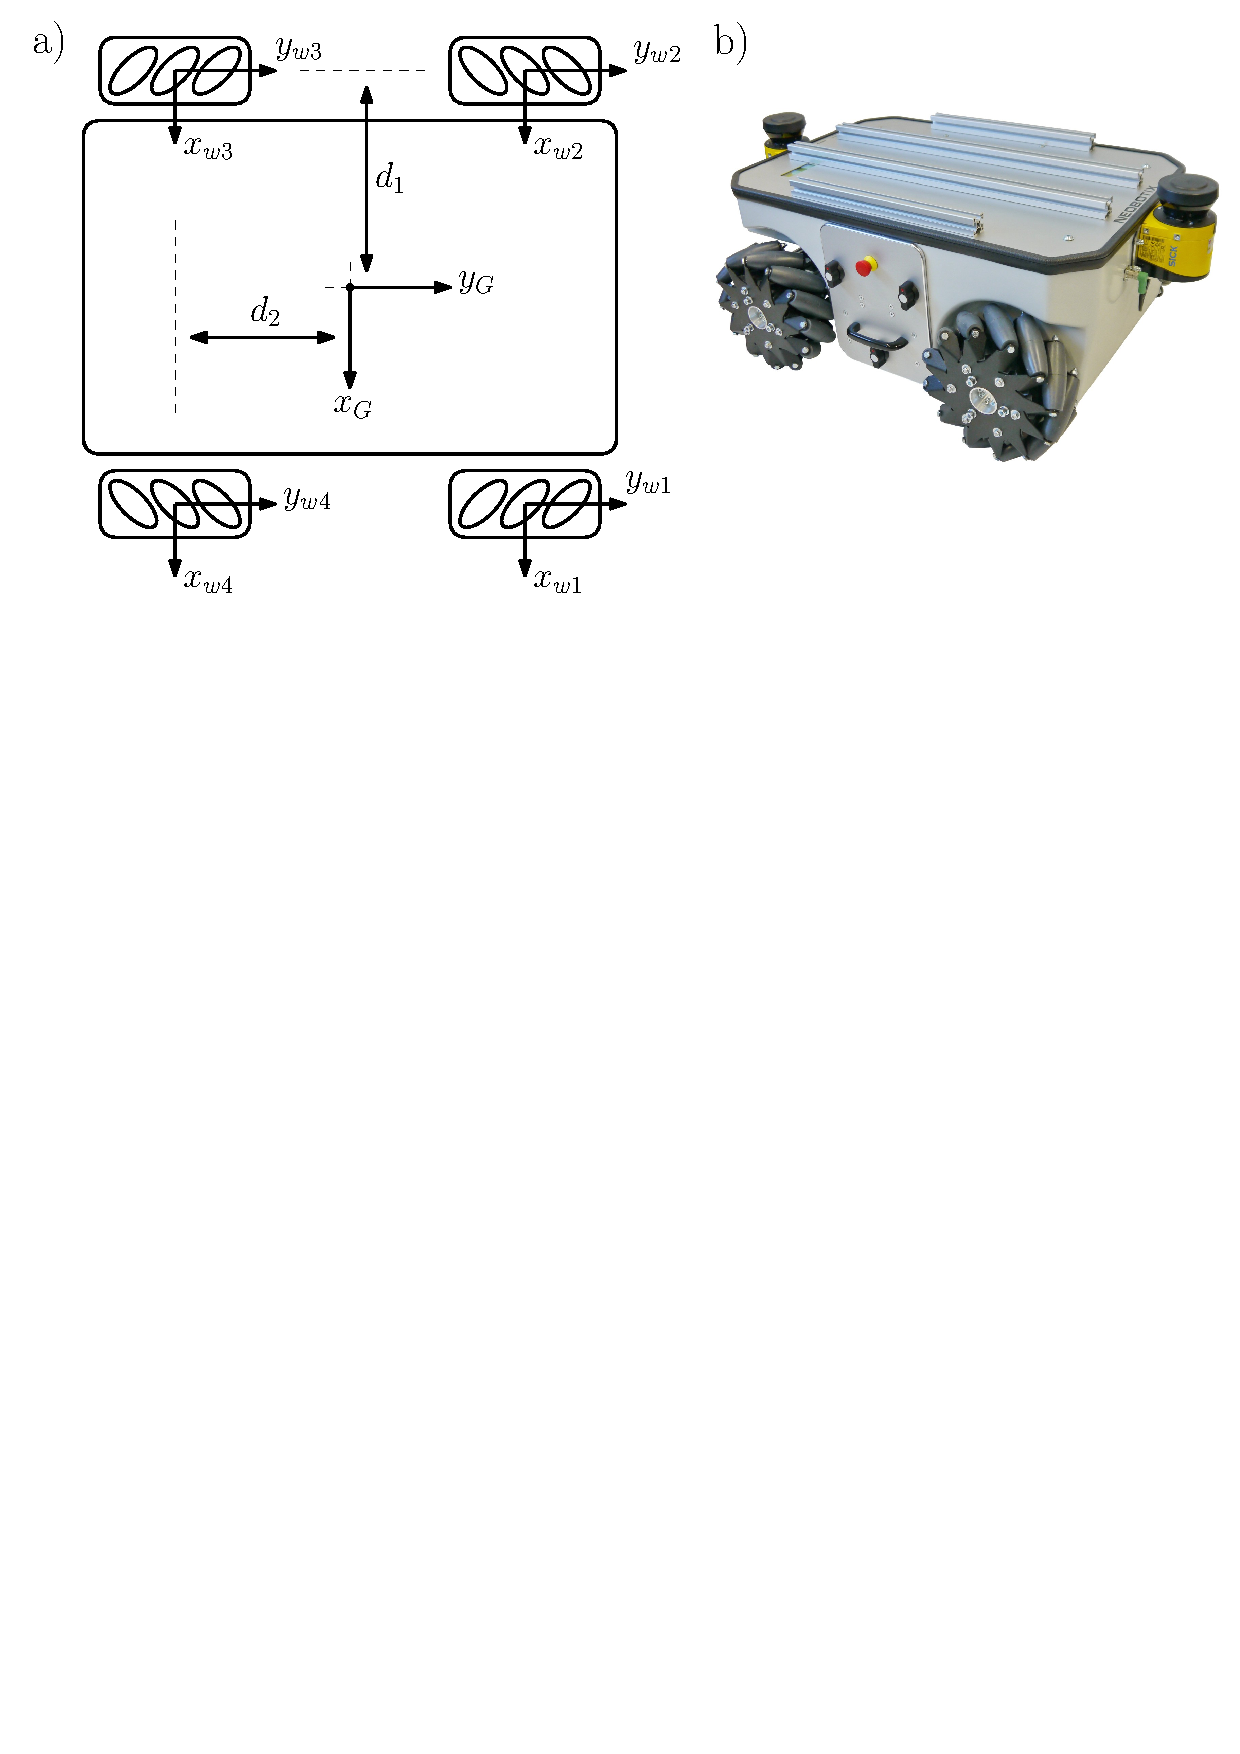
\includegraphics[width=0.7\linewidth]{omnib.pdf}
		%\caption{Оси координат двух соседних звеньев}
		\label{fig:scr11}
	\end{figure}
		\begin{minipage}[b]{0.9\textwidth}
Тогда соответствующий вектор скорости $v_{wi} = [\dot{x}_{wi}, \dot{y}_{wi}, \dot{\psi}_{wi}]^T$, выраженный в $O_{wi}$, определяется как:

\begin{equation*}
\begin{bmatrix}
\dot{x}_{wi}\\[1mm] \dot{y}_{wi}\\[1mm] \dot{\psi}_{wi}
\end{bmatrix} = 
\begin{bmatrix}
0 & r_i\sin(\alpha_i) & 0\\[1mm]
R_i & -r_i\cos(\alpha_i) & 0\\[1mm]
0 & 0 & 1
\end{bmatrix}
\begin{bmatrix}
\dot{q}_{ix}\\[1mm] \dot{q}_{iy}\\[1mm] \dot{q}_{iz}
\end{bmatrix}
\end{equation*}
		\end{minipage}
	\end{center}
\end{frame}

% 2
\begin{frame}{Всенаправленная колесная база}
	\begin{center}

\[
v_{b} = 
\begin{bmatrix}
\dot{x}_b\\[1mm] \dot{y}_b\\[1mm] \dot{\psi}_b
\end{bmatrix} = 
\begin{bmatrix}
\cos(\phi_{wi}^b) & -\sin(\phi_{wi}^b) & d_{wiy}^b\\[1mm]
\sin(\phi_{wi}^b) & \cos(\phi_{wi}^b) & -d_{wix}^b\\[1mm]
0 & 0 & 1
\end{bmatrix}
\begin{bmatrix}
\dot{x}_{wi}\\[1mm] \dot{y}_{wi}\\[1mm] \dot{\psi}_{wi}
\end{bmatrix}
\]
\[
\begin{bmatrix}
\dot{x}_b\\[1mm] \dot{y}_b\\[1mm] \dot{\psi}_b
\end{bmatrix} = 
\frac{R}{4}
\begin{bmatrix}
-1 & 1 & -1 & 1\\[1mm]
1 & 1 & 1 & 1\\[1mm]
\dfrac{1}{d_1+d_2} & \dfrac{-1}{d_1+d_2} & \dfrac{-1}{d_1+d_2} & \dfrac{1}{d_1+d_2}
\end{bmatrix}
\begin{bmatrix}
\dot{x}_{w1}\\[1mm] \dot{x}_{w2}\\[1mm] \dot{x}_{w3}\\[1mm] \dot{x}_{w4}\\[1mm]
\end{bmatrix}
\]

	\end{center}
\end{frame}

% 3
\begin{frame}{Учет проскальзывания}
	\begin{center}
		\begin{figure}[H]
		\center
		\renewcommand{\figurename}{}
		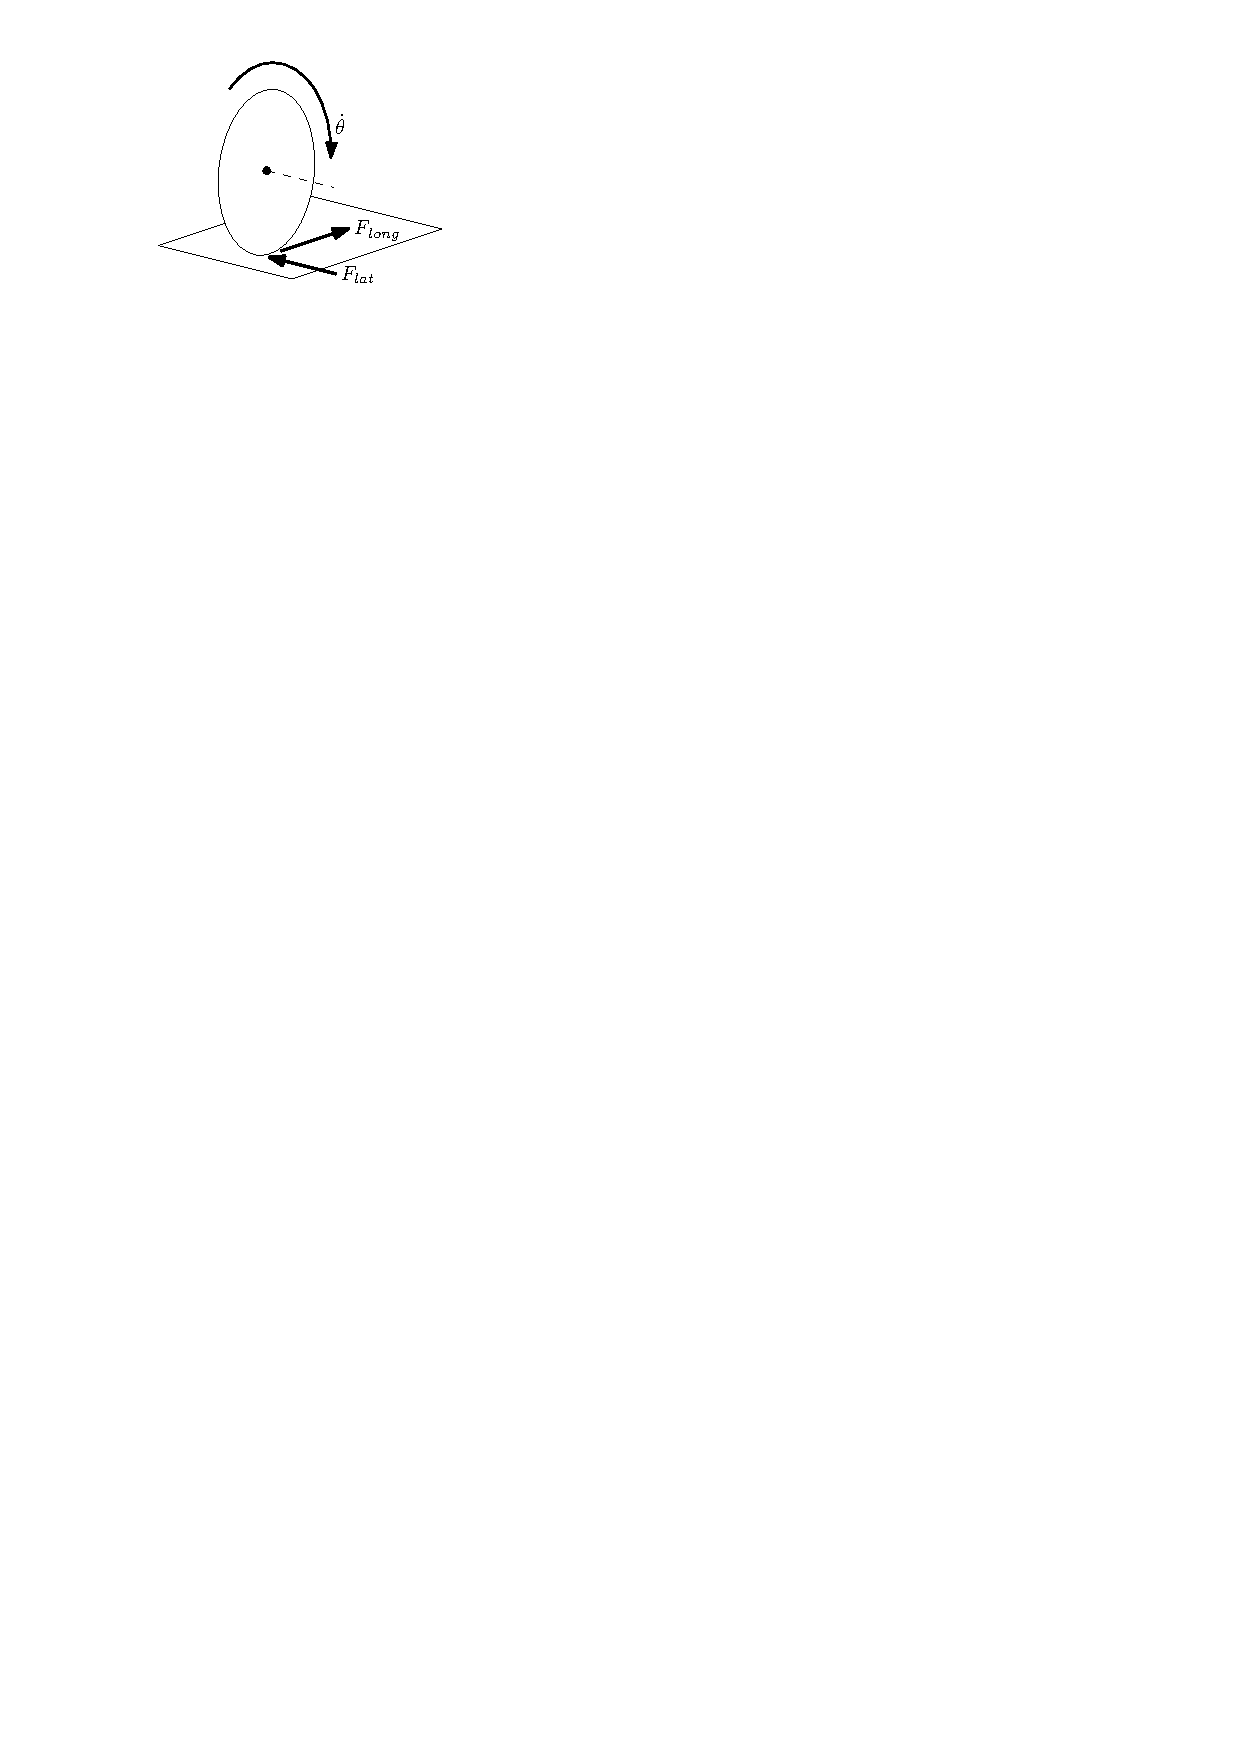
\includegraphics[width=0.4\linewidth]{wheelF.pdf}
		%\caption{Оси координат двух соседних звеньев}
		\label{fig:scr11}
	\end{figure}
	\vspace{-6mm}
\[
\upsilon_l^w = \dot{\theta{_l}}r - w_l = \dot{x}_b^w\cos(\psi) + \dot{y}_b^w\sin(\psi) - l\dot{\psi}
\]
\[
\upsilon_r^w = \dot{\theta{_r}}r - w_r = \dot{x}_b^w\cos(\psi) + \dot{y}_b^w\sin(\psi) + l\dot{\psi}
\]
\[
-\dot{x}^w_b\sin(\psi) + \dot{y}^w_b\cos(\psi) = z_r = z_l
\]
\[
q_b = 
\begin{bmatrix}
x^w_b& y^w_b& \psi& z_r& z_l& \upsilon_r^w& \upsilon_l^w& \theta_r& \theta_l
\end{bmatrix}
\]
	\end{center}
\end{frame}
\end{document}
